\documentclass[10pt]{article}
\usepackage[portuguese]{babel}
\usepackage[utf8]{inputenc}
\usepackage{color}
\usepackage{enumitem}
\usepackage{float}
\usepackage{graphicx}
\usepackage{minted}
\usepackage{geometry}
\usepackage{booktabs}
\geometry{%
    a4paper,
    total={150mm,257mm},
}
\usepackage{hyperref}
\hypersetup{%
    colorlinks=true,
    linkcolor=blue,
    filecolor=magenta,
    urlcolor=cyan,
}

\setlength{\arrayrulewidth}{0.3mm}
\setlength{\tabcolsep}{10pt}
% \setlength{\parindent}{0em}
\renewcommand{\arraystretch}{1.5}
% \renewcommand{\thesection}{}
% \renewcommand{\thesubsection}{}
% \renewcommand{\thesubsubsection}{}

\begin{document}
\begin{center}
    {\scshape Instituto Superior Técnico\par}
    \vspace{1cm}
    {\scshape\Large Applications and Computation for the Internet of Things\par}
    \vspace{1.5cm}
\end{center}
{\scshape\LARGE 3\textsuperscript{st} Lab Work: Internet of Sensors and Actuators}
\\
\begin{table}[h!]
    \centering
    \begin{tabular}{|l|l|p{10cm}|}
        \hline
        \multicolumn{3}{|l|}{Group: 12} \\[1.5ex] \hline
        Student 1 & 98380 & Dominika Florczykowska \\ [1.5ex]\hline
        Student 2 & 97144 & Pedro Mendes \\ [1.5ex]\hline
    \end{tabular}
\end{table}

\section{Describe the changes in the program developed in lab 2 (Sensing the
Real World) to port it to the new configuration with two controllers}

One important change made to maintain coherence between the code of the two
controllers is the addition of a \texttt{config.hpp} file where the values used
pins are set, this file can be used as a configuration file or as a
specification sheet for anyone trying to assemble this setup.

\inputminted{cpp}{../arduino/config.hpp}

This way, when writing the code of the either of the modules inconsistent led
to sensor choices can't be made.

\subsection{Describe any changes in the design pattern (such as changing
tasks in the round-robin loop)}\label{ss:design-pattern}

In the sensor loop, we are now constantly checking for the sensor analogue reading
and immediately sending the value via serial connection.

In the actuator loop, there are 2 tasks to run, the first one being later
broken up into 3 more.

The first task is trying to read from the serial port, if this fails (because
there was nothing to read or because the values read were invalid), then the sub
tasks are not run.

In the case where the read succeeds than an update function is run for each of
the 3 sensors.

The second task is to blink the green led, which means checking if the time turn
it off or on has passed and change it's state to the opposite.

It's important to note that in this design when one value changes, all actuators
are updated, this is only doable because there are so few actuators and updating
them is very simple, as well as some other optimizations made in other parts of
the project\textsuperscript{[\ref{p:temperature}] [\ref{ss:perf}]}.

We found this to simpler and allows for a higher data rate, as the amount of
data needed in each message is 8 bytes and requires nearly zero parsing. This
message is composed of 3 two byte values and a two byte error detection code.

If we had gone for a model where each message only pertains to one sensor, we
would need to exchange more data to transmit the same amount of information.
The message would need to be composed of 1 byte for de sensor identifier, 2 bytes
for the value, and 1 or 2 bytes for the error detection code, all this times 3
sensors for a total of 12--15 bytes (depending on the length of error code).
With the additional downside of needing to make 3 reads over the serial port
which can be even slower.

These design choices are only possible because:

\begin{itemize}
    \item The number of sensors is small;
    \item Their update functions are very short to compute;
    \item The fastest update rate of the blinking green led is slow enough.
\end{itemize}

Had any of these reasons been different we might have opted for more traditional
approach like the alternative explained above.

\subsection{Describe other implementation issues changed (implementation of
tasks)}

Two tasks suffered changes when transitioning to this model, the light detector
task did, however, not change at all.

\paragraph{Temperature Task}\label{p:temperature}

After reviewing the formula to convert an analogue read to degrees we came up
with 3 new options and benchmarked them to see which was best

The benchmark was done as follows:
\begin{quote}
    Every 10000 iterations write `r\textbackslash{}n' to the serial port. Run
    the program for 5 minutes and gather how many `r\textbackslash{}n' are
    written to the serial port.
\end{quote}

\begin{tabular}{llr}

    Version name  & formula                                           & Iterations/s
    \\\toprule
    float 1 (original) & $(((voltage / 1024.0) \times 5.0) - 0.5) \times 100.0$ & 12400\\
    float 2       & $((500.0 \times voltage) / 1024.0) - 50.0$             & 13066  \\
    short (16bit) & $((50 \times voltage) / 102) - 50$                     & 14600  \\
    long  (32bit) & $((500 \times (int32\_t) voltage) » 10) - 50$          & 15533 \\
\bottomrule

\end{tabular}

\begin{quote}
    \textbf{Note:} For the short (16bit) version, the formula had to be adapted
    to avoid overflows, hence the 50 instead of 500 and the 102 instead of the
    1024.
\end{quote}

Since the long (32bit) version was the fastest and the most accurate (using
integers that is) we decided to implement this one.


\paragraph{Potentiometer Task}

This task was changed so that the updating part was separated from the checking
when to swap on and off part.

The updating part can be seen in the \texttt{potentiometer} function and the
checking part can be seen in the \texttt{blink\_potentiometer} function, in the
actuator code (Subsection~\ref{ss:actuatorcode}).

\section{Controler \#1 program --- I2C master:}\label{ss:sensorcode}

\inputminted{cpp}{../arduino/sensor/sensor.hpp}

\inputminted[firstline=2]{cpp}{../arduino/sensor/sensor.ino}


\section{Controler \#2 program --- I2C slave:}\label{ss:actuatorcode}

\inputminted{cpp}{../arduino/actuators/actuators.hpp}

\inputminted[firstline=2]{cpp}{../arduino/actuators/actuators.ino}


\section{PC \#1 and \#2 configuration and programs:}

For communication between the arduinos we designed two programs in the
programming language Go. These act as mere communicators between the 2
controllers.

\subsection{The entry point of the command line program that interacts with the
controllers}

The first of these programs is connects to the serial port and to a relay
server. Through command line arguments this program can be used both for the
sensor and the actuator side. This program can also be used to ``mock'' a
controller by reading from and writing to a terminal, this was very useful
during testing.

This part of the code configures the application and the connects to the relay
server, telling it which kind of interface is connecting: sensor or actuator.

\inputminted[obeytabs=true,tabsize=2]{go}{../communication/serial_interface/main.go}

\subsection{The code to interact with a sensor}

The sensor part of this program does the parsing of the message sent from the
sensing controller to the packet format described in
Subsection~\ref{ss:design-pattern} and sending said packet to the relay server.

\inputminted[obeytabs=true,tabsize=2]{go}{../communication/serial_interface/sensor.go}

\subsection{The code to interact with the actuator side}

The actuator part reads from the relay server and writes to the serial port,
since the message format is the same, no parsing is done, only the error
code is checked as to ignore faulty messages. One final check is done before
sending the message, to avoid redundant messages it checks if this message is a
repeat of the last message and if so it's ignored. This avoids overloading the
controller with useless information.

\inputminted[obeytabs=true,tabsize=2]{go}{../communication/serial_interface/actuator.go}

\subsection{Relay server, establish communication between the two communication
programs}

The relay server serves as a mediator between the two interfaces, it stores the
most recent state and sends it to the actuator interface that is connected.

It also guarantees that the errors are sent from one interface to the other.

The relay only allows one actuator and one sensor to be connected at a time.

\inputminted[obeytabs=true,tabsize=2]{go}{../communication/relay_server/main.go}

\section{Evaluate the performance of the communication link}\label{ss:perf}

The program that interacts with the arduino on the actuator side is smart to not
write repeated messages consecutive, this way the arduino doesn't have to do
useless work and has more ``free time''. As such the data rates might seem a bit
low. But this is only because most of the data is redundant and not counted.
However, to give a sense of how much difference this makes, the code was
temporarily altered to not make this check.

\begin{tabular}{lrrr}
    Type            & Average (bytes/s) & Maximum (bytes/s) & Minimum (bytes/s) \\
    \toprule
    without repeats & 682               & 752               & 461 \\
    with repeats    & 805286            & 876945            & 521628 \\
    \bottomrule
\end{tabular}

\section{Design interfaces to detect failures of the LEDs and signal these
occurrences at the sensors side. (Consider that when a LED fails it behaves as an
open-circuit.)}

\subsection{Draw the circuits}

On the sensor side we have leds connected to the board which we use to signal an
error on the other side.

\begin{figure}[H]
    \centering
    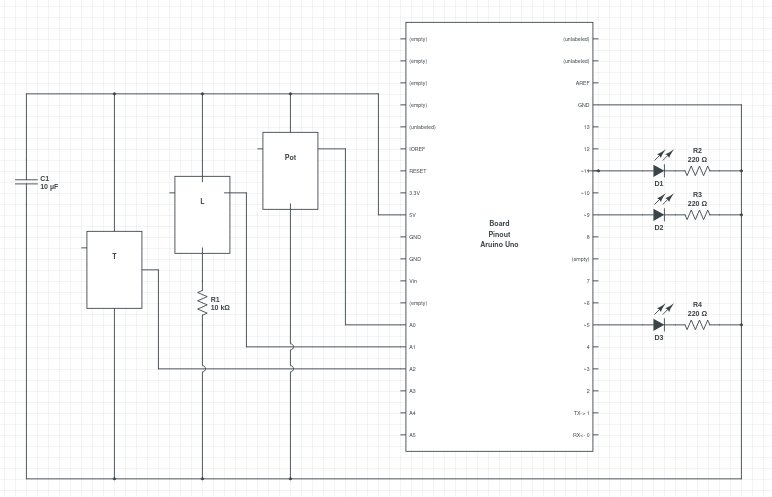
\includegraphics[width=\textwidth]{sensor2.png}
    \caption{Sensor}
\end{figure}

On the actuator side, we have the ``output'' of the LEDs being fed to analogue
pins so that their value can be inspected

\begin{figure}[H]
    \centering
    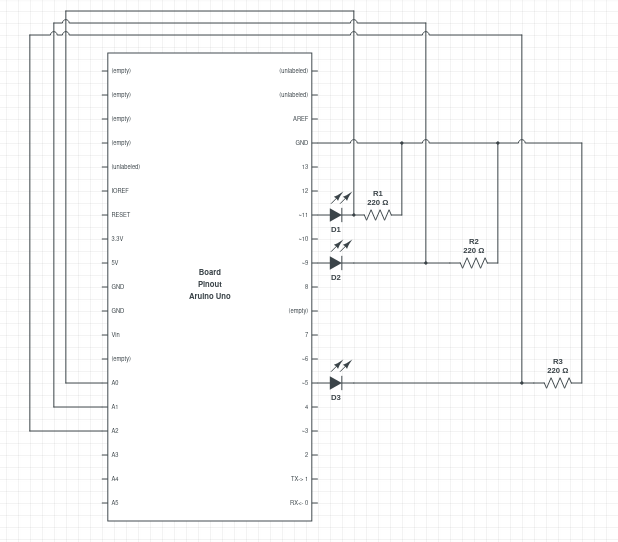
\includegraphics[width=\textwidth]{actuator.png}
    \caption{Actuator}
\end{figure}

Latency was not tested as it was very dependent on the speed of the internet
connection, if that is not taken in to account latency is negligible.

\subsection{Program the detection}

For yellow and green leds (the ones that are activated by digital writes) we
replaced the calls to \texttt{digitalWrite} with a
\texttt{checked\_digital\_write} function. For the red led we use a
\texttt{checked\_analog\_write} function, these are very similar except for the
for the fact that one does a digital write and the other an analogue write. The
used threshold passed to the test and report function is also different, this
value unfortunately couldn't not be thoroughly tested due to lack of time, it does
however work for most cases.

\inputminted[firstline=14, lastline=22]{cpp}{../arduino/actuators/actuators.hpp}

Which delegate the test and reporting this function:

\inputminted[firstline=29, lastline=35]{cpp}{../arduino/actuators/actuators.hpp}


\subsection{Describe any changes required in the communication interfaces}

The actuator side of the communication interface now has to also send things to
the sensor side, since TCP sockets are two way channels this wasn't very hard to
implement.

\end{document}
